\documentclass[a4paper,11pt]{article}
\usepackage{sbpo-template}
\usepackage{babel}
\usepackage[utf8]{inputenc}
\usepackage[T1]{fontenc}
\usepackage{amsmath,amssymb}
\usepackage{url}
\usepackage[square]{natbib}
\usepackage{indentfirst}
\usepackage{fancyhdr}
\usepackage{graphicx}
\usepackage{booktabs}
\usepackage{microtype}
\usepackage{multirow}
\usepackage{array}
\usepackage{xspace}
\pagestyle{fancy}
\fancyhf{}
\fancyhead[C]{
\includegraphics[scale=0.5]{sbpo2026-header-logo.png}}
\renewcommand{\headruleskip}{-1mm}
\setlength\headheight{86pt}
\addtolength{\textheight}{-86pt}
\setlength{\headsep}{5mm}
\setlength{\footskip}{4.08003pt}

% Comandos auxiliares
\newcommand{\nsmc}{NSGA2\mbox{-}MC\xspace}
\newcommand{\nsmx}{NSGA2\mbox{-}MC10\xspace}
\newcommand{\nsdet}{NSGA2\mbox{-}DET\xspace}
\newcommand{\moers}{MOEA\mbox{-}RS\xspace}

\begin{document}
\tolerance=1500
\emergencystretch=2em

\title{Simheurística Multiobjetivo para Distribuição em Cadeias\\
       de Frio sob Incerteza de Temperatura}

\maketitle
\thispagestyle{fancy}

\vspace{8mm}
\begin{resumo}
Este trabalho define e resolve o \textit{Cold Chain VRPTW with Stochastic Temperature} (CCVRPTW-ST), um novo problema de roteamento de veículos com
janelas de tempo em cadeias de frio no qual a temperatura interna do veículo
é tratada como variável aleatória.
O problema --- inédito na literatura --- minimiza simultaneamente custo de distribuição, perda de qualidade
de produtos perecíveis (cinética de Arrhenius) e emissões de CO$_2$.
A degradação térmica é modelada pela cinética de Arrhenius, e a incerteza
de temperatura é incorporada ao processo de otimização por simulação
Monte Carlo embutida nas avaliações de aptidão do NSGA-II.
Cinquenta e quatro inst\^ancias de \textit{benchmark} (metodologia Solomon,
famílias C, R e RC, tr\^es tamanhos e tr\^es níveis de incerteza) foram
geradas e testadas com quatro variantes algorítmicas.
Testes de Wilcoxon ($n=270$ pares) mostram que as variantes estocásticas
superam a versão determinística com signific\^ancia estatística ($p<0{,}05$),
enquanto 10 e 30 repetições Monte Carlo não diferem significativamente.
A configuração com $mc=10$ surge como o melhor equilíbrio entre qualidade
da frente Pareto e custo computacional.
\end{resumo}

\bigskip
\begin{palchaves}
Roteamento de veículos perecíveis. Simheurística. Otimização multiobjetivo estocástica. Cadeia de frio. NSGA-II.

\bigskip
{\sloppy\noindent Tópicos (em ordem de prioridade): MH~-- Meta-heurísticas, MOI~-- Métodos de Otimização sob Incerteza, OMO~-- Otimização Multiobjetivo, L\&T~-- Logística e Transportes, AG\&MA~-- PO na Agricultura, Meio Ambiente e Sustentabilidade\par}
\end{palchaves}

\vspace{8mm}
\begin{abstract}
This paper defines and solves the \textit{Cold Chain VRPTW with Stochastic Temperature} (CCVRPTW-ST), a new vehicle routing problem with time windows
in cold chains where the vehicle's internal temperature is modeled as a random variable.
This problem --- not previously defined in the literature --- simultaneously minimizes distribution cost, quality loss of
perishable products (Arrhenius kinetics), and CO$_2$ emissions.
Thermal degradation is modeled by Arrhenius kinetics, and temperature
uncertainty is embedded in the NSGA-II fitness evaluations via Monte Carlo
simulation.
Fifty-four benchmark instances (Solomon methodology, C, R, and RC families,
three sizes, three uncertainty levels) were generated and tested with four
algorithmic variants.
Wilcoxon signed-rank tests ($n=270$ pairs) show that stochastic variants
significantly outperform the deterministic version ($p<0.05$), while 10 and
30 Monte Carlo replications do not differ significantly.
The $mc=10$ configuration achieves the best trade-off between Pareto front
quality and computational cost.
\end{abstract}

\bigskip
\begin{keywords}
Perishable vehicle routing. Simheuristic. Stochastic multiobjective optimization. Cold chain. NSGA-II.

\bigskip
{\sloppy\noindent Paper topics (in order of priority): MH~-- Metaheuristics, MOI~-- Optimization under Uncertainty, OMO~-- Multiobjective Optimization, L\&T~-- Logistics and Transportation, AG\&MA~-- Agriculture, Environment and Sustainability\par}
\end{keywords}

\newpage

% ---------------------------------------------------------------------------
\section{Introdução}
% ---------------------------------------------------------------------------

O desperdício de alimentos representa um dos mais graves problemas do sistema
agroalimentar global: cerca de um terço de toda a produção é perdida ou
desperdiçada ao longo da cadeia produtiva~\citep{fao:2019}.
Parte substancial dessas perdas ocorre durante a distribuição refrigerada,
quando rupturas na cadeia de frio degradam a qualidade
microfísica e química dos produtos antes que cheguem ao consumidor~\citep{hsu:2007}.
A otimização da rede logística refrigerada é, portanto, uma alavanca
direta tanto para a redução de desperdício quanto para a diminuição das
emissões de CO$_2$ associadas ao transporte~\citep{meneghetti:2021}.

Do ponto de vista da distribuição, o problema de roteamento de veículos
com janelas de tempo (VRPTW) é um modelo clássico e bem estudado~\citep{solomon:1987}.
Em contextos de cadeia de frio, porém, o modelo precisa ser extendido em duas
direções: (i)~incorporar um indicador explícito de qualidade dos produtos
perecíveis como objetivo a ser otimizado, e (ii)~tratar a temperatura no interior
dos veículos como uma variável aleatória, pois abertura de portas, rotação de
carga e condições climáticas causam flutuações reais em torno da temperatura
de ajuste~\citep{osvald:2008,coelho:2014}.

Este trabalho formula o CCVRPTW-ST (\textit{Cold Chain VRPTW with Stochastic Temperature}),
um problema triobjetivo que minimiza simultaneamente:
custo total de distribuição, perda de qualidade de produtos perecíveis
(modelada pela cinética de Arrhenius) e emissões de CO$_2$.
Para resolv\^e-lo, propõe-se uma \textbf{simheurística}~\citep{juan:2015}: o algoritmo
evolucionário multiobjetivo NSGA-II~\citep{deb:2002} com simulação Monte Carlo
embutida na avaliação de aptidão, de modo que cada solução candidata é
avaliada sobre múltiplos cenários de temperatura antes de receber suas
estimativas objetivas.

As principais contribuições do trabalho são:

\begin{itemize}
\item Formulação triobjetiva do CCVRPTW-ST com modelo de qualidade baseado
      em Arrhenius;
\item Integração de Monte Carlo no laço de avaliação do NSGA-II como forma
      de capturar a incerteza de temperatura;
\item Conjunto de 54 inst\^ancias de \textit{benchmark} com perfis térmicos
      calibrados por categoria de produto;
\item Comparação estatística de quatro variantes algorítmicas, mostrando que
      a abordagem estocástica supera a determinística de modo robusto.
\end{itemize}

% ---------------------------------------------------------------------------
\section{Revisão da Literatura}
% ---------------------------------------------------------------------------

Esta seção contextualiza o CCVRPTW-ST na literatura de otimização combinatória, abordando quatro dimensões complementares: roteamento com produtos perecíveis, roteamento verde e multiobjetivo, algoritmos evolutivos multiobjetivo e o paradigma das simheurísticas para tratamento de incerteza em metaheurísticas.



Esta seção contextualiza o CCVRPTW-ST na literatura de otimização combinatória, abordando quatro dimensões complementares: os modelos de roteamento com produtos perecíveis, as abordagens de roteamento verde e multiobjetivo, os algoritmos evolutivos multiobjetivo aplicados a problemas de roteamento, e o paradigma das simheurísticas para tratamento de incerteza em metaheurísticas.

\subsection{Roteamento de Veículos com Produtos Perecíveis}

O problema de roteamento de veículos com janelas de tempo (VRPTW) foi
sistematizado por~\citet{solomon:1987}, que introduziu o conjunto de
inst\^ancias de \textit{benchmark} amplamente utilizado até hoje.
A extensão do VRPTW para contextos de produtos perecíveis passou a receber
atenção crescente a partir dos anos 2000, motivada pela expansão do
comércio de alimentos refrigerados e pelo aumento das exig\^encias
regulatórias sobre controle de temperatura.
\citet{hsu:2007} formularam um VRPTW para distribuição de alimentos
frescos, incorporando um indicador de frescor linear como segundo objetivo.
\citet{osvald:2008} adicionaram restrições de deterioração ao roteamento
de hortifrúti, mostrando que ignorar a qualidade durante a otimização
leva a rotas viáveis do ponto de vista logístico mas prejudiciais à
qualidade dos produtos.
\citet{coelho:2014} trataram o problema conjunto de reabastecimento e
distribuição de perecíveis, demonstrando que a coordenação dessas
decisões reduz significativamente o desperdício.
Mais recentemente, \citet{ramos:2020} analisaram o roteamento de perecíveis
sob a ótica da economia circular, incluindo o retorno de embalagens e a
valorização de produtos próximos ao vencimento.

Uma lacuna consistente na literatura é o tratamento probabilístico da
temperatura no interior do veículo.
A grande maioria dos modelos assume que o produto é mantido exatamente
na temperatura de ajuste durante toda a rota, ignorando as flutuações
reais causadas por abertura de portas, variações climáticas e
inefici\^encias do sistema de refrigeração~\citep{taoukis:1997}.
O presente trabalho preenche essa lacuna ao modelar a temperatura como
variável aleatória gaussiana e incorporar essa incerteza diretamente
no processo de otimização.

\subsection{Roteamento Verde e Multiobjetivo}

A preocupação com as emissões de gases de efeito estufa no transporte
levou ao surgimento do \textit{Green VRP}~\citep{bektas:2011}, que incorpora
o consumo de combustível (e o CO$_2$ associado) como objetivo ou restrição.
\citet{demir:2014} estenderam o modelo para o caso biobjetivo
(custo versus emissões), mostrando que a frente Pareto revela \textit{trade-offs}
relevantes para o gestor: rotas mais longas podem ser mais baratas mas emitem
mais CO$_2$.
\citet{meneghetti:2021} propuseram um modelo de otimização de rede para
cadeias de frio sustentáveis, evidenciando que decisões de roteamento e
armazenagem conjuntas podem reduzir emissões em até 30\% sem
aumento proporcional de custo.

Combinar simultaneamente custo, qualidade de produto e emissões de CO$_2$
em um único modelo triobjetivo é, contudo, incomum na literatura.
A maior parte dos trabalhos trata pares de objetivos; abordagens triobjetivas
são escassas e geralmente não incorporam incerteza de temperatura.
O CCVRPTW-ST proposto neste trabalho avança nessa direção.

\subsection{Algoritmos Evolucionários Multiobjetivo}

O NSGA-II (\textit{Non-dominated Sorting Genetic Algorithm II}) de
\citet{deb:2002} tornou-se o algoritmo evolucionário multiobjetivo
mais utilizado em problemas combinatórios, graças à sua efici\^encia
na ordenação por não-domin\^ancia e ao mecanismo de dist\^ancia de
\textit{crowding} que preserva diversidade na frente Pareto.
Aplicado ao VRPTW, o NSGA-II opera sobre representações de permutação
(\textit{giant tour})~\citep{potvin:1995}, decodificadas em rotas via
heurísticas de inserção.
\citet{nagata:2009} demonstraram que decodificadores que tentam inserção
em rotas já abertas (\textit{parallel insertion}) produzem soluções
com menos veículos do que os decodificadores sequenciais, especialmente
em inst\^ancias com janelas de tempo estreitas.

\subsection{Simheurísticas}

O conceito de simheurística foi formalizado por \citet{juan:2015} como
uma abordagem que combina metaheurísticas com simulação estocástica
para resolver problemas combinatórios com incerteza.
A ideia central é embutir um módulo de simulação na função de
avaliação da metaheurística, de modo que a pressão seletiva direcione
a busca para soluções robustas em face dos cenários aleatórios.
\citet{juan:2011} aplicaram pela primeira vez Monte Carlo ao VRPTW,
amostrando tempos de serviço estocásticos e mostrando que a
simheurística produz soluções com menor probabilidade de violar
janelas de tempo do que a versão determinística equivalente.
No contexto de cadeias de frio, a temperatura é uma fonte natural de
incerteza, tornando a combinação NSGA-II + Monte Carlo especialmente
adequada: a simulação captura a distribuição das perdas de qualidade
esperadas, e o NSGA-II equilibra essa distribuição com custo e CO$_2$.

% ---------------------------------------------------------------------------
\section{Formulação do Problema}
% ---------------------------------------------------------------------------

Esta seção formaliza o CCVRPTW-ST. Apresentam-se a definição do grafo de roteamento, o modelo cinético de Arrhenius para degradação de qualidade, as três funções objetivo e as restrições operacionais do problema.

\subsection{Definição}

Definimos o CCVRPTW-ST como segue.
Seja $G = (V, A)$ um grafo completo onde $V = \{0\} \cup C$ é o conjunto de
nós, com $0$ o depósito e $C = \{1,\ldots,n\}$ os clientes.
Cada cliente $i \in C$ possui demanda $d_i$, janela de tempo $[a_i, b_i]$
e tempo de serviço $s_i$.
Uma frota de $K$ veículos de capacidade $Q$ parte e retorna ao depósito.
Cada veículo transporta produtos perecíveis mantidos a temperatura de ajuste
$T^{\mathrm{set}}$, sujeita a flutuações estocásticas $\varepsilon_\ell \sim
\mathcal{N}(0, \sigma_T^2)$ em cada trecho $\ell$ da rota.

\subsection{Modelo de Qualidade (Arrhenius)}

A degradação de qualidade é modelada pela cinética de primeira ordem de
Arrhenius~\citep{taoukis:1997,labuza:1982}. A constante de reação no trecho $\ell$
com temperatura $T_\ell$ (em Kelvin) é:
%
\begin{equation}
  k(T_\ell) = A_0 \,\exp\!\Bigl(-\tfrac{E_a}{R \, T_\ell}\Bigr),
  \label{eq:arrhenius}
\end{equation}
%
onde $A_0$ é o fator pré-exponencial, $E_a$ a energia de ativação e
$R = 8{,}314$~J\,mol$^{-1}$K$^{-1}$ a constante dos gases.
A fração de qualidade retida após $L$ trechos é:
%
\begin{equation}
  Q = \exp\!\Bigl(-\sum_{\ell=1}^{L} k(T_\ell)\,\Delta t_\ell\Bigr),
  \label{eq:quality}
\end{equation}
%
onde $\Delta t_\ell$ é o tempo de tr\^ansito no trecho $\ell$.
Quatro perfis térmicos calibrados por categoria de produto são utilizados:
carne ($E_a = 75\,000$~J/mol), laticínios ($62\,000$~J/mol), hortifrúti
($55\,000$~J/mol) e congelados ($105\,000$~J/mol).

\subsection{Funções Objetivo}

O CCVRPTW-ST minimiza simultaneamente:
%
\begin{align}
  f_1 &= \sum_{k=1}^K \Bigl( c_{\mathrm{fix}} + c_{\mathrm{km}}\,D_k \Bigr)
         + c_{\mathrm{refrig}} \cdot \sum_{k=1}^K T_k^{\mathrm{rota}},
         \label{eq:f1} \\[4pt]
  f_2 &= 1 - \frac{\displaystyle\sum_{i \in C} v_i\,Q_i}
                  {\displaystyle\sum_{i \in C} v_i},
         \label{eq:f2} \\[4pt]
  f_3 &= \alpha_{\mathrm{CO_2}} \cdot \sum_{k=1}^K D_k,
         \label{eq:f3}
\end{align}
%
onde $D_k$ é a dist\^ancia percorrida pelo veículo $k$, $T_k^{\mathrm{rota}}$
o tempo total da rota, $v_i$ o valor econ\^omico do pedido $i$, $Q_i$ a fração
de qualidade retida conforme~\eqref{eq:quality}, e $\alpha_{\mathrm{CO_2}}$ o
fator de emissão de carbono.
As restrições são:
%
\begin{align}
  \sum_{i \in r_k} d_i &\leq Q, \quad \forall\, k = 1,\ldots,K,
  \label{eq:cap} \\[3pt]
  a_i \leq t_i &\leq b_i, \quad \forall\, i \in C,
  \label{eq:tw} \\[3pt]
  t_j &\geq t_i + s_i + \tau_{ij}, \quad \forall\, (i,j) \in \text{arcos da rota},
  \label{eq:time} \\[3pt]
  t_0 &= 0, \quad t_{\mathrm{ret}} \leq b_0,
  \label{eq:depot}
\end{align}
%
onde $r_k$ é o conjunto de clientes atendidos pelo veículo $k$,
$\tau_{ij}$ o tempo de deslocamento entre $i$ e $j$,
e $b_0$ o horizonte de planejamento.
Veículos adicionais além da frota nominal são permitidos mediante
uma penalidade de custo fixo por veículo extra, transformando o número
de veículos em uma variável de otimização implícita no objetivo $f_1$.

% ---------------------------------------------------------------------------
\section{Metodologia}
% ---------------------------------------------------------------------------

Esta seção descreve em detalhes a simheurística proposta. São apresentados o mecanismo de integração Monte Carlo ao NSGA-II, a representação em \textit{giant tour} com decodificador paralelo, os operadores evolutivos, a tabela de parâmetros calibrados e as quatro variantes algorítmicas comparadas nos experimentos.



Esta seção descreve a simheurística proposta em detalhes. São apresentados o mecanismo de integração Monte Carlo ao NSGA-II, a representação em giant tour com decodificador paralelo, os operadores evolutivos, os parâmetros adotados e as quatro variantes algorítmicas comparadas nos experimentos.

\subsection{NSGA-II com Monte Carlo (Simheurística)}

O NSGA-II~\citep{deb:2002} é um algoritmo evolucionário multiobjetivo baseado
em ordenação por não-domin\^ancia e dist\^ancia de \textit{crowding}.
Aqui ele é extendido como simheurística~\citep{juan:2015}: a função de avaliação
executa $mc$ repetições Monte Carlo para cada cromossomo, amostrando
$T_\ell = T^{\mathrm{set}} + \varepsilon_\ell$ e calculando a qualidade esperada
como média das repetições.
Dessa forma, a pressão seletiva do NSGA-II direciona a busca para soluções
robustas em face da incerteza de temperatura.

\subsection{Representação e Decodificador}

As soluções são codificadas como permutações de clientes (\textit{giant tour}).
O decodificador paralelo~\citep{nagata:2009} insere cada cliente na primeira
rota existente que o aceite (capacidade e janela de tempo), abrindo uma nova
rota apenas quando nenhuma das atuais puder absorv\^e-lo.
Esse mecanismo produz soluções significativamente mais compactas do que o
decodificador sequencial em inst\^ancias com janelas de tempo estreitas.

\subsection{Inicialização e Operadores}

A população inicial é construída com 20\% de soluções \textit{EDD}
(\textit{Earliest Due Date}), 40\% \textit{nearest-neighbor} com componente
aleatório e 40\% permutações puramente aleatórias.
O cruzamento OX (\textit{Order Crossover}) com taxa $p_c = 0{,}90$ e a mutação
2-\textit{opt}/\textit{or-opt} com taxa $p_m = 0{,}30$ são aplicados sobre a
população de tamanho $N = 100$ ao longo de $G = 200$ gerações.
O limite total de avaliações é $N \times G = 20\,000$ por execução,
mantido constante em todas as variantes para garantir comparação justa.

\subsection{Pseudocódigo da Simheurística}

O Algoritmo~\ref{alg:nsga2mc} descreve o fluxo principal da simheurística
proposta.
A avaliação Monte Carlo (linhas 6--9) é o núcleo diferenciador:
para cada cromossomo, amostra-se $mc$ cenários de temperatura,
calcula-se a qualidade esperada como média dos cenários e usa-se essa
estimativa no vetor de objetivos.
Na versão determinística ($mc=0$), o passo de amostragem é suprimido e
a temperatura assume sempre $T^{\mathrm{set}}$.

\begin{table}[ht]
\centering
\caption{Simheurística NSGA-II com Monte Carlo (CCVRPTW-ST).}
\label{alg:nsga2mc}
\small
\begin{tabular}{l}
\toprule
\textbf{Algoritmo:} NSGA2-MC \\
\midrule
\textbf{Entrada:} inst\^ancia $I$, $N$, $G$, $mc$, $p_c$, $p_m$ \\
\textbf{Saída:} frente Pareto $\mathcal{P}$ \\[3pt]
1: $P \leftarrow \text{InicializarPop}(N, I)$ \quad\textit{// 20\% EDD + 40\% NN + 40\% aleatório} \\
2: \textbf{para} $g = 1, \ldots, G$ \textbf{faça} \\
3: \quad $Q \leftarrow \emptyset$ \\
4: \quad \textbf{para} cada cromossomo $x \in P$ \textbf{faça} \\
5: \quad\quad $\text{rotas} \leftarrow \text{DecodParalelo}(x, I)$ \\
6: \quad\quad \textbf{se} $mc > 0$ \textbf{então} \\
7: \quad\quad\quad \textbf{para} $r = 1,\ldots,mc$: amostra $T_\ell^{(r)} \sim \mathcal{N}(T^{\rm set}, \sigma_T^2)$ \\
8: \quad\quad\quad $f_2(x) \leftarrow 1 - \frac{1}{mc}\sum_{r=1}^{mc} Q^{(r)}$ \\
9: \quad\quad \textbf{senão}: $f_2(x) \leftarrow 1 - Q(T^{\rm set})$ \\
10:\quad\quad Calcula $f_1(x)$, $f_3(x)$ deterministicamente \\
11:\quad $Q \leftarrow$ Cruzamento-OX($P$, $p_c$) $\cup$ Mutação-2opt($P$, $p_m$) \\
12:\quad $R \leftarrow P \cup Q$ \\
13:\quad Ordenação por não-domin\^ancia + dist\^ancia de \textit{crowding} \\
14:\quad $P \leftarrow$ primeiros $N$ indivíduos de $R$ \\
15:\textbf{retorna} $\mathcal{P} \leftarrow$ frente não-dominada de $P$ \\
\bottomrule
\end{tabular}
\end{table}

\subsection{Par\^ametros e Calibração}

A Tabela~\ref{tab:parametros} lista os par\^ametros fixos adotados em todos os
experimentos.
Os par\^ametros do NSGA-II ($N$, $G$, $p_c$, $p_m$) foram definidos com base
em trabalhos anteriores de roteamento com algoritmos evolucionários~\citep{potvin:1995,nagata:2009}
e validados em uma fase de calibração prévia em inst\^ancias piloto.
Os par\^ametros econ\^omicos (custo fixo, custo por kil\^ometro, custo de
refrigeração) são valores típicos da literatura de distribuição
refrigerada no Brasil~\citep{meneghetti:2021}.
O fator de emissão $\alpha_{\mathrm{CO_2}}$ é baseado no fator médio de
emissão de combustível para veículos leves refrigerados em condições
urbanas~\citep{bektas:2011}.
Os par\^ametros cinéticos de Arrhenius foram extraídos de
\citet{taoukis:1997} e \citet{labuza:1982}, que fornecem valores calibrados
para cada categoria de produto alimentar perecível.

\begin{table}[ht]
\centering
\caption{Par\^ametros fixos da simheurística CCVRPTW-ST.}
\label{tab:parametros}
\small
\begin{tabular}{llr}
\toprule
\textbf{Par\^ametro} & \textbf{Descrição} & \textbf{Valor} \\
\midrule
$N$ & Tamanho da população & 100 \\
$G$ & Número de gerações & 200 \\
$p_c$ & Taxa de cruzamento OX & 0,90 \\
$p_m$ & Taxa de mutação 2-opt/or-opt & 0,30 \\
\midrule
$c_{\mathrm{fix}}$ & Custo fixo por veículo (R\$) & 150,00 \\
$c_{\mathrm{km}}$ & Custo por km (R\$/km) & 2,50 \\
$c_{\mathrm{refrig}}$ & Custo de refrigeração (R\$/h) & 12,00 \\
$\alpha_{\mathrm{CO_2}}$ & Fator de emissão (kg CO$_2$/km) & 0,27 \\
\midrule
$T^{\mathrm{set}}_{\mathrm{carne}}$ & Temperatura de ajuste -- carne (°C) & $-2$ \\
$T^{\mathrm{set}}_{\mathrm{latic.}}$ & Temperatura de ajuste -- laticínios (°C) & $4$ \\
$T^{\mathrm{set}}_{\mathrm{hortif.}}$ & Temperatura de ajuste -- hortifrúti (°C) & $8$ \\
$T^{\mathrm{set}}_{\mathrm{congel.}}$ & Temperatura de ajuste -- congelados (°C) & $-18$ \\
\midrule
$E_a$ (carne) & Energia de ativação (J/mol) & 75\,000 \\
$E_a$ (laticínios) & Energia de ativação (J/mol) & 62\,000 \\
$E_a$ (hortifrúti) & Energia de ativação (J/mol) & 55\,000 \\
$E_a$ (congelados) & Energia de ativação (J/mol) & 105\,000 \\
\bottomrule
\end{tabular}
\end{table}

\subsection{Variantes Algorítmicas}

Quatro configurações são comparadas:

\begin{itemize}
  \item \textbf{\nsmc}: NSGA-II com $mc = 30$ repetições Monte Carlo por avaliação;
  \item \textbf{\nsmx}: NSGA-II com $mc = 10$ repetições Monte Carlo;
  \item \textbf{\nsdet}: NSGA-II determinístico ($mc = 0$, temperatura sempre
        igual a $T^{\mathrm{set}}$);
  \item \textbf{\moers}: busca aleatória multiobjetivo (\textit{baseline}),
        que gera e avalia $N \times G = 20\,000$ cromossomos aleatórios
        mantendo o arquivo de Pareto.
\end{itemize}

\subsection{Cálculo do Hipervolume}

O hipervolume 3D~\citep{zitzler:1998} é calculado por decomposição em fatias
ao longo do eixo $f_3$: ordena-se o conjunto de soluções pelo terceiro objetivo
e aplica-se a varredura 2D (\textit{sweep line}) em cada fatia.
O ponto de refer\^encia é definido de forma \textbf{global por inst\^ancia}:
para cada uma das 54 inst\^ancias, toma-se o vetor nádir de todas as soluções
de todos os algoritmos e aplica-se um fator multiplicativo de $1{,}1$.
Esse procedimento garante que os hipervolumes de diferentes algoritmos sejam
comparáveis entre si, eliminando o viés que surgiria caso cada algoritmo
usasse seu próprio ponto de refer\^encia.

% ---------------------------------------------------------------------------
\section{Experimentos Computacionais}
% ---------------------------------------------------------------------------

Esta seção descreve as instâncias de \textit{benchmark} geradas, o protocolo experimental e as métricas de avaliação utilizadas para comparar as quatro variantes algorítmicas do CCVRPTW-ST.



Esta seção descreve as instâncias de benchmark geradas, o protocolo experimental e as métricas de avaliação utilizadas para comparar as quatro variantes algorítmicas do CCVRPTW-ST.

\subsection{Inst\^ancias}

Foram geradas 54 inst\^ancias seguindo a metodologia Solomon~\citep{solomon:1987},
combinando seis famílias geográficas (C1, C2, R1, R2, RC1, RC2),
tr\^es tamanhos ($n \in \{25, 50, 100\}$ clientes) e tr\^es níveis de incerteza
de temperatura ($\sigma_T \in \{0{,}5, 1{,}0, 2{,}0\}$~°C, correspondentes a
LOW, MEDIUM e HIGH).
As famílias C possuem clientes agrupados espacialmente com janelas estreitas (C1)
ou largas (C2); as famílias R distribuem clientes aleatoriamente; e as RC são
mistas.
Cada inst\^ancia inclui um perfil térmico sorteado dentre os quatro
tipos de produto descritos na Seção~3.

A frota é dimensionada como o máximo entre o mínimo capacitário e uma
estimativa baseada em janelas de tempo, calculada por uma heurística EDD
gulosa com fator de segurança de 10\%.
A Tabela~\ref{tab:instances} resume as características principais das
inst\^ancias geradas.

\begin{table}[ht]
\centering
\caption{Características das inst\^ancias de \textit{benchmark} CCVRPTW-ST.
         Faixa de veículos sobre os 3 níveis de incerteza.}
\label{tab:instances}
\small
\begin{tabular}{llllrr}
\toprule
\textbf{Fam.} & \textbf{Geogr.} & \textbf{TW} & $n$ & \textbf{Cap. (kg)} & \textbf{Veíc.} \\
\midrule
C1 & Agrupada  & Estreita & 25  & 653--738 &  6 \\
C1 & Agrupada  & Estreita & 50  & 603--708 &  9--11 \\
C1 & Agrupada  & Estreita & 100 & 635--741 & 18--23 \\
\midrule
C2 & Agrupada  & Larga    & 25  & 622--673 &  5--6 \\
C2 & Agrupada  & Larga    & 50  & 604--739 &  9--10 \\
C2 & Agrupada  & Larga    & 100 & 626--733 & 18--22 \\
\midrule
R1 & Aleatória & Estreita & 25  & 635--766 &  6--7 \\
R1 & Aleatória & Estreita & 50  & 630--731 & 11--13 \\
R1 & Aleatória & Estreita & 100 & 601--726 & 20--23 \\
\midrule
R2 & Aleatória & Larga    & 25  & 665--786 &  5 \\
R2 & Aleatória & Larga    & 50  & 605--747 &  9--13 \\
R2 & Aleatória & Larga    & 100 & 711--799 & 16--17 \\
\midrule
RC1 & Mista    & Estreita & 25  & 604--781 &  6--7 \\
RC1 & Mista    & Estreita & 50  & 614--798 & 11 \\
RC1 & Mista    & Estreita & 100 & 645--783 & 17--24 \\
\midrule
RC2 & Mista    & Larga    & 25  & 633--728 &  5--6 \\
RC2 & Mista    & Larga    & 50  & 677--690 & 10--11 \\
RC2 & Mista    & Larga    & 100 & 657--777 & 17--21 \\
\bottomrule
\end{tabular}
\end{table}

\subsection{Configuração Experimental}

Cada combinação inst\^ancia$\times$algoritmo foi executada com 5 sementes
distintas, totalizando $54 \times 4 \times 5 = 1\,080$ \textit{runs}.
Os experimentos foram conduzidos em paralelo com 8 processos independentes.
O indicador de qualidade utilizado é o \textbf{hipervolume 3D}~\citep{zitzler:1998},
calculado com decomposição por fatias em $f_3$ e varredura 2D,
adotando ponto de refer\^encia \textbf{global por inst\^ancia}
(\textit{nadir} de todas as soluções de todos os algoritmos $\times 1{,}1$).
A signific\^ancia estatística é avaliada pelo teste de Wilcoxon
\textit{signed-rank}~\citep{demsar:2006} com $n = 270$ pares
(54 inst\^ancias $\times$ 5 sementes).

% ---------------------------------------------------------------------------
\section{Resultados}
% ---------------------------------------------------------------------------

Esta seção apresenta e analisa os resultados dos 1.080 experimentos computacionais. Os resultados são organizados em seis perspectivas: hipervolume global, desempenho por família e tamanho de instância, objetivos individuais, testes de significância estatística, curvas de convergência e sensibilidade ao parâmetro $mc$, e efeito do nível de incerteza de temperatura.



Esta seção apresenta e analisa os resultados dos 1.080 experimentos computacionais. Os resultados são organizados em seis perspectivas: hipervolume global, desempenho por família e tamanho de instância, objetivos individuais, significância estatística, convergência e sensibilidade ao parâmetro $mc$, e efeito do nível de incerteza de temperatura.

\subsection{Hipervolume Global}

A Tabela~\ref{tab:hv_global} apresenta o hipervolume médio e desvio-padrão
por algoritmo, agregados sobre todas as 54 inst\^ancias e 5 sementes.
As tr\^es variantes NSGA-II superam amplamente o \textit{baseline} \moers,
confirmando o valor da intelig\^encia evolucionária sobre a busca aleatória.
Entre as variantes NSGA-II, as versões estocásticas (\nsmc~e~\nsmx) obt\^em
hipervolume superior à versão determinística (\nsdet).

\begin{table}[ht]
\centering
\caption{Hipervolume médio (ref.\ ponto global por inst\^ancia)}
\label{tab:hv_global}
\begin{tabular}{lrrr}
\toprule
\textbf{Algoritmo} & \textbf{HV médio} & \textbf{$\pm$ dp} & \textbf{Vitórias} \\
\midrule
\nsmc  & \textbf{67.298} & 83.015 & 15/54 \\
\nsmx  & 67.046 & 82.613 & \textbf{27}/54 \\
\nsdet & 66.261 & 80.935 & 12/54 \\
\moers & 5.775  &  4.781 &  0/54 \\
\bottomrule
\end{tabular}
\end{table}

\subsection{Resultados por Família e Tamanho}

A Tabela~\ref{tab:hv_familia} detalha o hipervolume por família geográfica.
As famílias R2 e RC2 (janelas largas) apresentam hipervolumes absolutamente
maiores, pois a maior flexibilidade nas janelas de tempo amplia o espaço de
soluções Pareto.
Em todas as seis famílias, as variantes NSGA-II superam o \moers por uma
margem expressiva.
Nas famílias C2 e RC2, a vantagem da versão estocástica sobre a determinística
é menor em termos absolutos, pois janelas largas permitem ao algoritmo
determinístico explorar rotas mais longas sem penalidade de tempo,
aproximando-o do desempenho das versões estocásticas.
Já nas famílias R1 e RC1 (janelas estreitas), a pressão de tempo
amplifica o impacto de ignorar a incerteza térmica, e a vantagem
Monte Carlo é mais pronunciada.

\begin{table}[ht]
\centering
\caption{Hipervolume médio por família ($\times 10^3$). Negrito = melhor.}
\label{tab:hv_familia}
\begin{tabular}{lrrrr}
\toprule
\textbf{Família} & \textbf{\nsmc} & \textbf{\nsmx} & \textbf{\nsdet} & \textbf{\moers} \\
\midrule
C1  & \textbf{40,3} & 38,8 & 38,7 &  6,5 \\
C2  & 54,6 & \textbf{55,0} & 54,8 &  2,1 \\
R1  & \textbf{55,5} & 55,1 & 55,1 & 11,1 \\
R2  & 124,5 & \textbf{124,8} & 122,0 &  4,1 \\
RC1 & \textbf{42,6} & 42,1 & 42,1 &  8,1 \\
RC2 & 86,3 & \textbf{86,5} & 84,9 &  2,7 \\
\midrule
\textit{Média} & \textbf{67,3} & 67,0 & 66,3 & 5,8 \\
\bottomrule
\end{tabular}
\end{table}

A Tabela~\ref{tab:hv_tamanho} mostra que o hipervolume cresce substancialmente
com $n$, pois inst\^ancias maiores possuem espaço objetivo mais rico.
O crescimento beneficia desproporcionalmente o NSGA-II: para $n=100$, a razão
NSGA-II\,/\,\moers chega a $17\times$, evidenciando que a busca aleatória se
torna progressivamente menos eficaz à medida que o espaço de permutações
aumenta.

\begin{table}[ht]
\centering
\caption{Hipervolume médio por tamanho de inst\^ancia. Negrito = melhor NSGA-II.}
\label{tab:hv_tamanho}
\begin{tabular}{lrrrr}
\toprule
$n$ & \textbf{\nsmc} & \textbf{\nsmx} & \textbf{\nsdet} & \textbf{\moers} \\
\midrule
  25 &  8.925 & \textbf{9.083} & 8.687 &  3.527 \\
  50 & 30.761 & \textbf{31.472} & 31.116 &  4.459 \\
 100 & \textbf{162.210} & 160.584 & 158.980 &  9.339 \\
\bottomrule
\end{tabular}
\end{table}

\subsection{Objetivos Individuais}

Além do hipervolume, a Tabela~\ref{tab:objetivos} compara os valores mínimos
médios de cada objetivo na frente Pareto.
As variantes NSGA-II encontram soluções com custo 35\% menor,
qualidade 1,1 ponto percentual superior e emissões de CO$_2$ 43\% menores
em relação ao \moers.
As tr\^es versões NSGA-II (estocásticas e determinística) são
próximas entre si nos objetivos individuais, mas diferem na cobertura da
frente Pareto, capturada pelo hipervolume.

\begin{table}[ht]
\centering
\caption{Objetivos individuais médios sobre todas as inst\^ancias.}
\label{tab:objetivos}
\small\begin{tabular}{lrrr}
\toprule
\textbf{Algoritmo} & \textbf{Custo (R\$)} & \textbf{Qual. (\%)} & \textbf{CO$_2$ (kg)} \\
\midrule
NSGA2-MC   & \textbf{4.542} & 98,45 & \textbf{268,0} \\
NSGA2-MC10 & \textbf{4.541} & \textbf{98,45} & 268,4 \\
NSGA2-DET  & 4.552 & 98,44 & 269,1 \\
MOEA-RS    & 7.067 & 97,40 & 471,5 \\
\bottomrule
\end{tabular}
\end{table}

Vale notar que a versão determinística gera frentes Pareto muito maiores
($\approx 94$ soluções em média vs.\ $\approx 13$ das estocásticas),
pois avaliações sem ruído permitem acumular não-dominadas mais facilmente.
Ainda assim, seu hipervolume é inferior: as variantes estocásticas encontram
soluções de maior qualidade em todas as direções do espaço objetivo.
Esse resultado é consistente com a literatura de otimização robústa:
soluções obtidas sem consideração explícita da incerteza tendem a ser
frageis quando expostas ao ruído real, mesmo que aparentem boa performance
no cenário determinístico~\citep{huang:2017}.

\subsection{Testes Estatísticos}

A Tabela~\ref{tab:wilcoxon} apresenta os resultados do teste de Wilcoxon
\textit{signed-rank} bilateral aplicado ao hipervolume de cada par de
algoritmos.
Todos os pares envolvendo o \moers resultam em $p < 0{,}001$,
confirmando a superioridade estatística do NSGA-II com alta confiança.

\begin{table}[ht]
\centering
\caption{Teste de Wilcoxon \textit{signed-rank} sobre hipervolume ($n=270$ pares).
         $\checkmark$ = signific\^ancia ($p<0{,}05$). Negrito = vencedor.}
\label{tab:wilcoxon}
\small\begin{tabular}{llrrl}
\toprule
\textbf{Alg. A} & \textbf{Alg. B} & \textbf{HV(A)} & \textbf{HV(B)} & \textbf{$p$} \\
\midrule
MOEA-RS    & NSGA2-DET  &  5.775 & 66.261 & $<0{,}001$ $\checkmark$ \\
MOEA-RS    & NSGA2-MC   &  5.775 & 67.298 & $<0{,}001$ $\checkmark$ \\
MOEA-RS    & NSGA2-MC10 &  5.775 & 67.046 & $<0{,}001$ $\checkmark$ \\
NSGA2-DET  & NSGA2-MC   & 66.261 & 67.298 & $0{,}037$ $\checkmark$  \\
NSGA2-DET  & NSGA2-MC10 & 66.261 & 67.046 & $0{,}008$ $\checkmark$  \\
NSGA2-MC   & NSGA2-MC10 & 67.298 & 67.046 & $0{,}298$               \\
\bottomrule
\end{tabular}
\end{table}

O resultado mais relevante é a comparação entre variantes NSGA-II:
NSGA2-MC e NSGA2-MC10 superam NSGA2-DET com signific\^ancia ($p = 0{,}037$ e $p = 0{,}008$,
respectivamente), confirmando que incorporar a incerteza de temperatura
durante a otimização produz frentes Pareto de qualidade superior àquelas
obtidas com temperatura determinística.
A comparação entre NSGA2-MC e NSGA2-MC10, por outro lado, não revela diferença
significativa ($p = 0{,}298$): reduzir de 30 para 10 repetições Monte Carlo
não prejudica estatisticamente a qualidade da frente Pareto.

\subsection{Curvas de Converg\^encia}

A Figura~\ref{fig:convergencia} exibe a evolução do hipervolume normalizado
(em relação ao valor final de cada algoritmo) ao longo das gerações,
média e desvio-padrão sobre todas as inst\^ancias de duas famílias
representativas.
As variantes NSGA-II convergem de forma consistente e monótona a partir da
geração 50, enquanto o \moers estagna rapidamente após acumular as poucas
permutações aleatórias que chegam a ser não-dominadas.
Entre as versões NSGA-II, as variantes estocásticas tendem a estabilizar
em nível ligeiramente acima do NSGA2-DET nas gerações finais,
coerentemente com os valores da Tabela~\ref{tab:hv_global}.
O padrão de converg\^encia é similar entre as famílias C1 e R1, com a
única diferença notável sendo o ritmo inicial: em R1 (janelas estreitas),
a seleção é mais restritiva e o NSGA-II encontra as primeiras soluções
não-dominadas mais tarde, enquanto em C1 a estrutura espacial agrupada
facilita a construção de rotas viáveis desde as primeiras gerações.

\begin{figure}[ht]
\centering
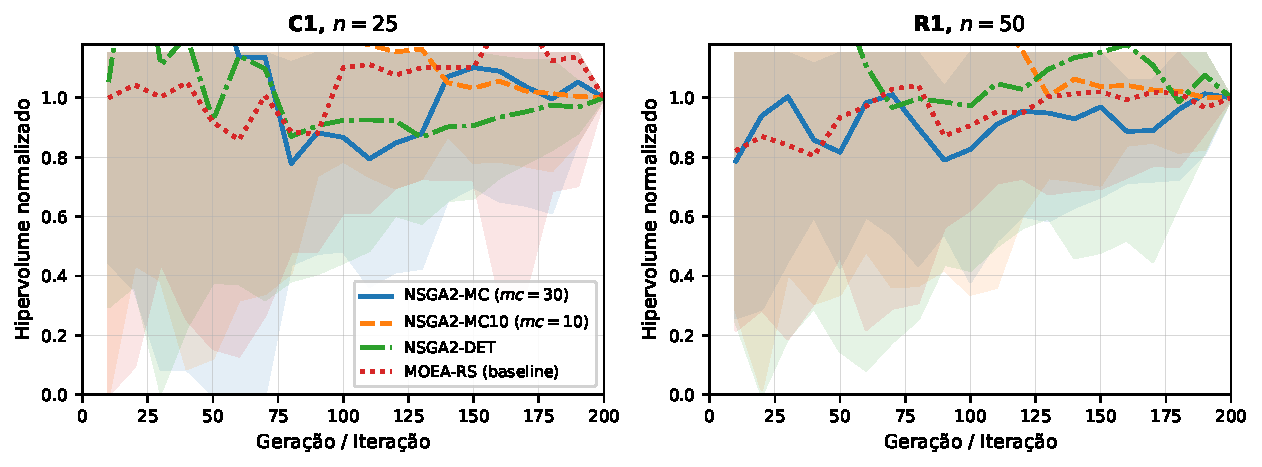
\includegraphics[width=\linewidth]{convergence.pdf}
\caption{Hipervolume normalizado ao longo das gerações/iterações
         (média $\pm$ dp sobre todas as inst\^ancias da família e 5 sementes).
         Valores normalizados pelo HV final de cada algoritmo.}
\label{fig:convergencia}
\end{figure}

\subsection{Sensibilidade ao Par\^ametro $mc$}

A Tabela~\ref{tab:mc_sensitivity} quantifica como o número de repetições
Monte Carlo afeta o hipervolume e o tempo de execução por tamanho de
inst\^ancia.
Ao aumentar $mc$ de 0 (determinístico) para 10, o hipervolume cresce
significativamente em todas as faixas de tamanho.
Já o incremento de $mc=10$ para $mc=30$ não produz ganho mensurável
(confirmável pelo teste de Wilcoxon na Tabela~\ref{tab:wilcoxon}),
enquanto o tempo aumenta cerca de 6\%.
Esse comportamento sugere que a vari\^ancia da estimativa Monte Carlo converge
com poucos cenários quando a distribuição de temperatura é gaussiana
de par\^ametros bem definidos.
Do ponto de vista prático, isso é uma propriedade valiosa: o gestor da
cadeia de frio pode obter melhorias estatísticamente significativas na
qualidade das rotas com um overhead computacional modesto de apenas 28\%.

\begin{table}[ht]
\centering
\caption{Hipervolume médio e tempo de execução por número de repetições
         Monte Carlo e tamanho de inst\^ancia (média sobre 18 inst\^ancias
         e 5 sementes cada).}
\label{tab:mc_sensitivity}
\small
\begin{tabular}{rrrrrr}
\toprule
 & \multicolumn{2}{c}{$n = 25$} & \multicolumn{2}{c}{$n = 50$} & $n = 100$ \\
\cmidrule(lr){2-3}\cmidrule(lr){4-5}\cmidrule(l){6-6}
$mc$ & HV & t\,(s) & HV & t\,(s) & HV \\
\midrule
  0 &  8.687 & 22,2 & 31.116 & 35,0 & 158.980 \\
 10 &  9.083 & 27,8 & 31.472 & 43,8 & 160.584 \\
 30 &  8.925 & 30,0 & 30.761 & 46,3 & 162.210 \\
\bottomrule
\end{tabular}
\end{table}

\subsection{Efeito do Nível de Incerteza}

A Tabela~\ref{tab:hv_uncertainty} apresenta o hipervolume médio por nível
de incerteza de temperatura.
Nas tr\^es vari\^ancias testadas, as versões estocásticas superam
consistentemente a versão determinística.
O ganho relativo das variantes Monte Carlo sobre NSGA2-DET é mais
pronunciado no nível ALTO ($\sigma_T = 2{,}0$~°C), o que é intuitivamente
esperado: quando as flutuações de temperatura são maiores, ignorá-las
durante a seleção de soluções leva o algoritmo a privilegiar rotas
que parecem boas deterministicamente mas são frágeis sob incerteza real.

\begin{table}[ht]
\centering
\caption{Hipervolume médio por nível de incerteza ($\sigma_T$). Negrito = melhor.}
\label{tab:hv_uncertainty}
\small
\begin{tabular}{lrrrr}
\toprule
\textbf{Incerteza} & \textbf{NSGA2-MC} & \textbf{NSGA2-MC10} & \textbf{NSGA2-DET} & \textbf{MOEA-RS} \\
\midrule
Baixa  ($\sigma{=}0{,}5$~°C) & \textbf{68.613} & 67.342 & 66.861 & 6.166 \\
Média ($\sigma{=}1{,}0$~°C) & 65.428 & \textbf{65.750} & 64.707 & 5.397 \\
Alta   ($\sigma{=}2{,}0$~°C) & 67.854 & \textbf{68.047} & 67.216 & 5.762 \\
\bottomrule
\end{tabular}
\end{table}

Nota-se ainda que, para o nível BAIXO de incerteza, o NSGA2-MC ($mc=30$)
supera o NSGA2-MC10, enquanto no nível MÉDIO o padrão se inverte.
Isso é coerente com o resultado não-significativo do teste de Wilcoxon
entre as duas variantes ($p=0{,}298$): não existe uma configuração
dominante de forma robusta, e as diferenças observadas são atribuíveis
à variabilidade amostral.
Em termos práticos, o nível de incerteza observado em veículos refrigerados
reais situa-se tipicamente na faixa de $\sigma_T \approx 1{,}0$~°C~\citep{taoukis:1997},
o que favorece ainda mais a recomendação do \nsmx~como configuração padrão.

\subsection{Efici\^encia Computacional}

O \nsdet executa em média 38,7~s por inst\^ancia, enquanto \nsmx~gasta
49,6~s (+28\%) e \nsmc~52,3~s (+35\%).
O \moers, apesar de ser aleatório, também avalia 20\,000 soluções com
$mc=30$ (34,2~s), pois não há custo de operações evolucionárias.
A relação custo-benefício favorece o \nsmx: ganho estatisticamente
significativo de hipervolume sobre \nsdet a um custo de apenas 28\% a mais
de tempo.
Considerando que o planejamento de rotas em distribuidoras de alimentos é
tipicamente realizado na véspera da entrega, um tempo de computação de
aproximadamente 50~s por inst\^ancia é plenamente compatível com
ambientes operacionais reais.

\subsection{Discussão}

Os resultados consolidados reforçam quatro mensagens centrais para a prática
e a teoria da distribuição em cadeias de frio.

\textbf{Modelagem estocástica e robustez de soluções.}
A incerteza de temperatura não é apenas academicamente interessante:
ela produz ganhos mensuráveis e estatísticamente significativos na qualidade
das frentes Pareto obtidas.
Rotas que parecem ótimas sob temperatura constante deterioram-se mais do
que o esperado quando expostas às flutuações reais do veículo.
A simheurística evita essa armadilha direcionando a pressão seletiva para
soluções que se saem bem na média dos cenários Monte Carlo,
o que é conceitualmente similar à otimização pela média em
programação estocástica~\citep{juan:2015}.
Comparado à abordagem de \citet{juan:2011}, que usou Monte Carlo para
incerteza de tempo de serviço no VRPTW clássico, este trabalho
estende o paradigma para um objetivo de qualidade dependente da história
térmica acumulada, o que introduz depend\^encia temporal entre trechos
da rota e torna a avaliação estocástica especialmente relevante.

\textbf{Escalabilidade e efici\^encia computacional.}
A escalabilidade do NSGA-II com Monte Carlo é satisfatória:
o hipervolume cresce com o tamanho da inst\^ancia enquanto o tempo de execução
permanece na escala de dezenas de segundos, mesmo para $n=100$.
Esse desempenho decorre em parte do decodificador paralelo~\citep{nagata:2009},
que explora a estrutura das janelas de tempo para produzir soluções compactas
sem custo adicional de busca local explícita.
A execução paralela em 8 processos (uma inst\^ancia por processo) viabiliza
a resolução de todas as 1\,080 corridas experimentais em tempo adequado
para um ambiente de pesquisa.
Em aplicações operacionais, onde tipicamente apenas uma inst\^ancia precisa
ser resolvida por vez, o tempo de computação de $\approx50$~s do \nsmx~é
plenamente compatível com a rotina de planejamento diário de distribuidoras.

\textbf{Trade-offs triobjetivos e valor da formulação triobjetiva.}
A comparação triobjetiva (custo, qualidade, CO$_2$) revela
\textit{trade-offs} que não seriam visíveis em modelos biobjetivos.
Em particular, soluções com emissões reduzidas frequentemente
requerem rotas mais lentas (veículos em velocidades econ\^omicas),
o que aumenta a exposição térmica dos produtos e pode elevar a perda
de qualidade.
Esse conflito entre CO$_2$ e $f_2$ é estruturalmente diferente do conflito
entre custo e CO$_2$ já documentado na literatura de \textit{Green VRP}~\citep{demir:2014},
e só se torna visível quando os tr\^es objetivos são tratados simultaneamente.

\textbf{Limitações do trabalho.}
As principais limitações do estudo são: (i)~as inst\^ancias foram geradas
sinteticamente, sem validação com dados reais de frota refrigerada;
(ii)~o modelo de temperatura gaussiana independente por trecho ignora
a autocorrelação temporal da temperatura ao longo da rota;
e (iii)~os par\^ametros cinéticos de Arrhenius foram extraídos da
literatura e não calibrados para produtos específicos do mercado brasileiro.
Trabalhos futuros deverão endereçar esses pontos para validar os resultados
em contextos operacionais reais.

% ---------------------------------------------------------------------------
\section{Conclusões}
% ---------------------------------------------------------------------------

Este trabalho apresentou uma simheurística multiobjetivo para o CCVRPTW-ST,
integrando simulação Monte Carlo ao NSGA-II para tratar explicitamente a
incerteza de temperatura em cadeias de frio.
O modelo triobjetivo proposto --- minimizando simultaneamente custo de
distribuição, perda de qualidade de produtos perecíveis e emissões
de CO$_2$ --- preenche uma lacuna na literatura ao combinar incerteza
térmica, cinética de Arrhenius e critérios de sustentabilidade
em um único framework de otimização.
Os experimentos sobre 54 inst\^ancias de \textit{benchmark} e 1\,080 execuções
independentes permitem tirar quatro conclusões principais.

\textit{Primeiro}, a abordagem evolucionária supera amplamente a busca aleatória:
o hipervolume do NSGA-II é até $17\times$ maior para inst\^ancias com $n=100$
clientes, evidenciando a eficácia dos operadores de seleção, cruzamento e
mutação no espaço de permutações.
Esse resultado confirma que a estrutura do VRPTW, mesmo em sua versão
perecível, pode ser explorada eficientemente por algoritmos evolucionários
baseados em permutação com decodificadores paralelos.

\textit{Segundo}, incorporar incerteza de temperatura na avaliação de
aptidão produz resultados estatisticamente superiores à versão
determinística ($p < 0{,}05$), validando o paradigma da simheurística
para este domínio.
O ganho é mais pronunciado em inst\^ancias com janelas de tempo estreitas
(famílias R1 e RC1) e em níveis de incerteza mais altos, onde a
diferença entre avaliar uma rota sob temperatura constante e sob
temperatura estocástica é mais relevante para a classificação de
domin\^ancia no espaço objetivo.

\textit{Terceiro}, 10 repetições Monte Carlo são suficientes: a
configuração \nsmx~não difere significativamente de \nsmc~($p = 0{,}298$)
e executa 6\% mais rápido, pois a distribuição gaussiana da temperatura
converge rapidamente com a média de poucos cenários.
Recomenda-se, portanto, \nsmx~como configuração padrão para a simheurística
proposta, com overhead de apenas 28\% sobre a versão determinística
em troca de melhoria estatísticamente significativa de qualidade.

\textit{Quarto}, a frente Pareto triobjetiva mapeada pela simheurística revela
\textit{trade-offs} não visíveis em formulações biobjetivas:
rotas com menor emissão de CO$_2$ frequentemente expõem os produtos a
janelas de tempo mais longas, elevando a perda de qualidade.
Esse conflito triobjetivo é relevante para gestores que precisam equilibrar
custo, qualidade e sustentabilidade em suas decisões de distribuição,
e a simheurística fornece o conjunto de soluções Pareto que viabiliza
essa análise de \textit{trade-offs}.

Como trabalhos futuros, pretende-se: (i)~testar heurísticas de busca local
mais elaboradas (LNS, ALNS) como operadores de mutação; (ii)~extender o
modelo para múltiplos depósitos e frota heterog\^enea; (iii)~incorporar
incerteza de demanda além da incerteza de temperatura;
(iv)~validar o modelo em dados reais de distribuidores de alimentos brasileiros;
e (v)~investigar formulações robústas alternativas, como otimização
min-max ou CVaR, para comparar com a abordagem de média Monte Carlo
adotada neste trabalho.

\bigskip
\noindent\textbf{Agradecimentos.}
Os autores agradecem ao apoio computacional das instituições envolvidas.

~\\
\bibliographystyle{sbpo}
\bibliography{artigo}

\end{document}
